\subsection{Company growth}

\begin{frame}{Bob's company is being very successfull...}
  \begin{center}
    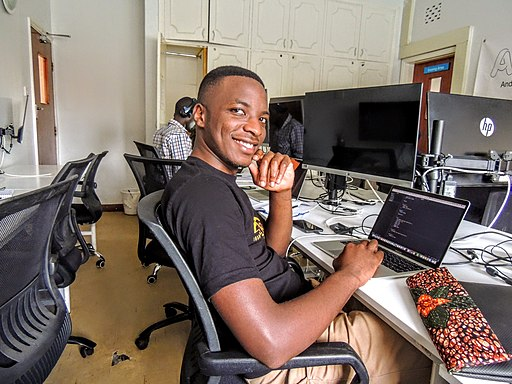
\includegraphics[width=.7\textwidth]{./assets/bob.jpeg}
  \end{center}
\end{frame}

\begin{frame}{A company growth... so its architecture}
  \begin{center}
    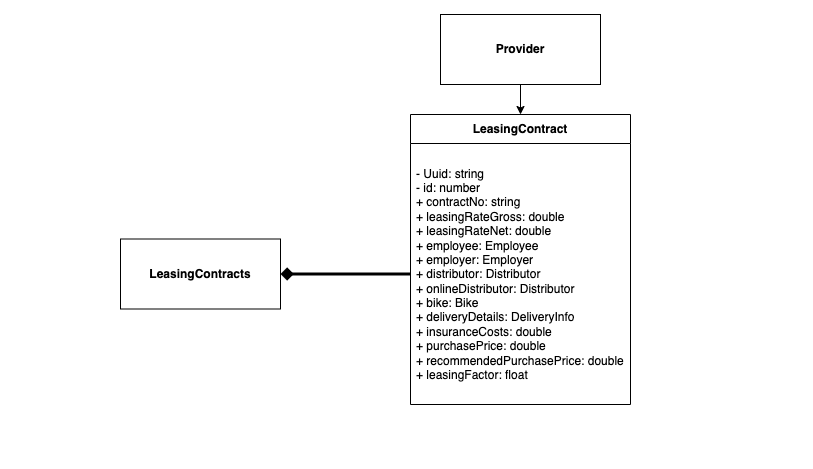
\includegraphics[scale=.5]{./assets/model1}
  \end{center}
\end{frame}

\begin{frame}{A company growth... so its architecture}
  \begin{center}
    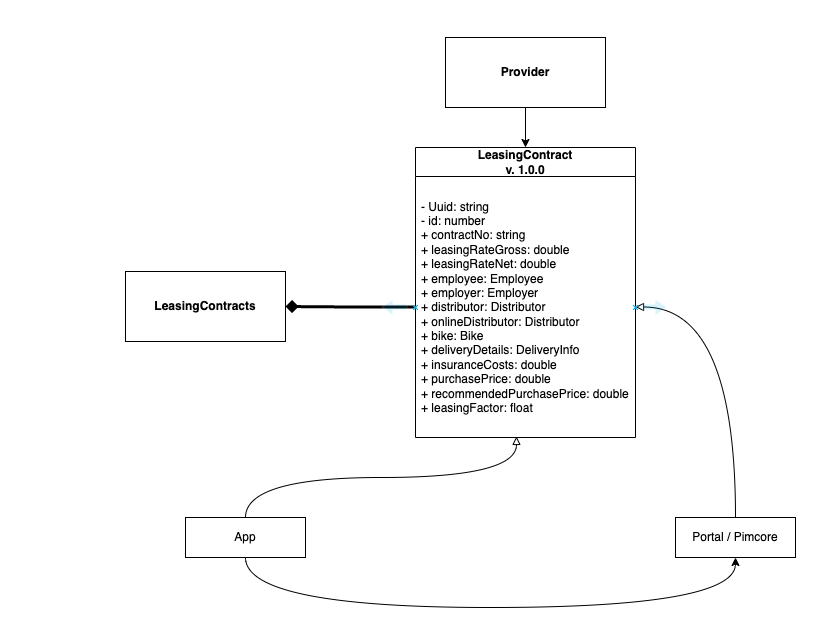
\includegraphics[scale=.35]{./assets/model2}
  \end{center}
\end{frame}


\begin{frame}{A company growth... so its architecture}
  \begin{center}
    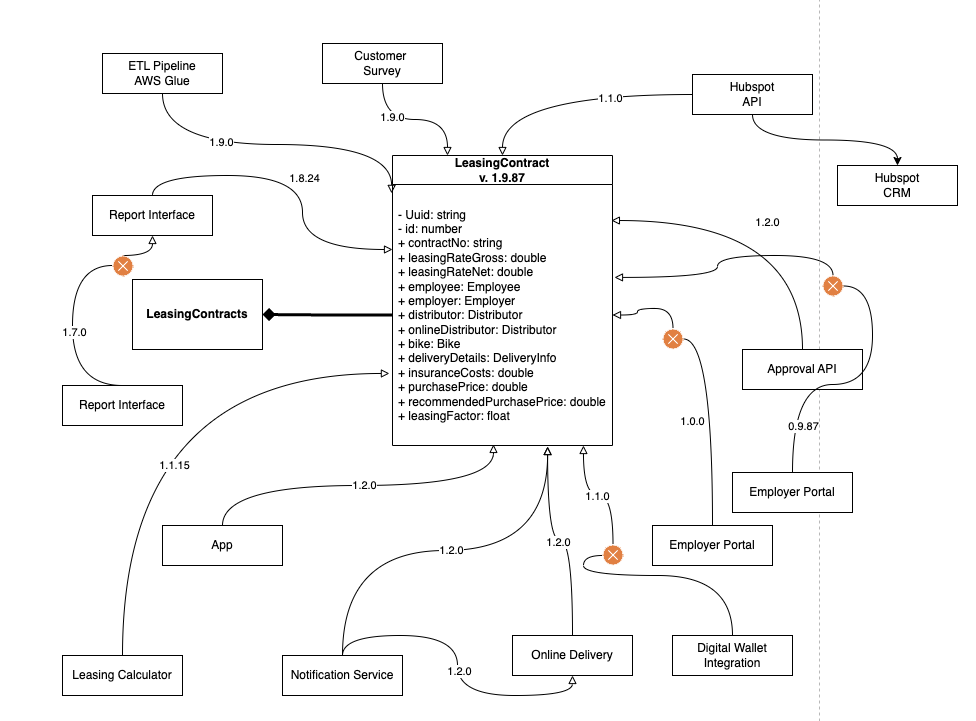
\includegraphics[scale=.3]{./assets/model3}
  \end{center}
\end{frame}


\begin{frame}{Bob is happy...}
  \begin{center}
    
\includegraphics[scale=.45]{./assets/chaos}
  \end{center}
\end{frame}

\begin{frame}{The Problem...}
  \begin{shadequote}
    \hspace{1cm} Every time we touch one service, all the others break :(
  \end{shadequote}
  \begin{columns}
    \begin{column}{0.6\textwidth}
      \begin{itemize}
        \item Dependency hell
        \item Devs don't have confidence in deploying changes
        \begin{itemize}
          \item Consequences of changes are hard to track
          \item Distributed architectures are hard to test
        \end{itemize}
      \end{itemize}
    \end{column}
    \begin{column}{0.4\textwidth}
      
\includegraphics[scale=.3]{./assets/sad_dev.jpeg}
    \end{column}
  \end{columns}
  \end{frame}

\begin{frame}{Architecture example: Online Delivery}
  \begin{center}
    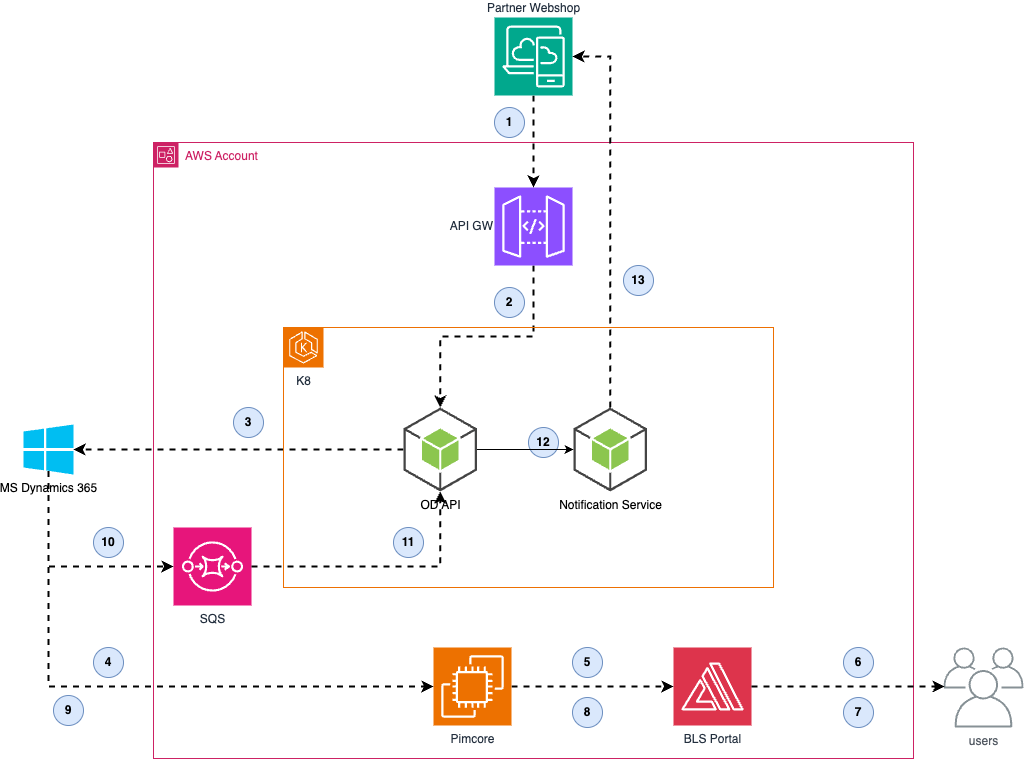
\includegraphics[scale=.3]{./assets/od.png}
  \end{center}
\end{frame}

\begin{frame}{Architecture example: Leasing Calculator}
  \begin{center}
    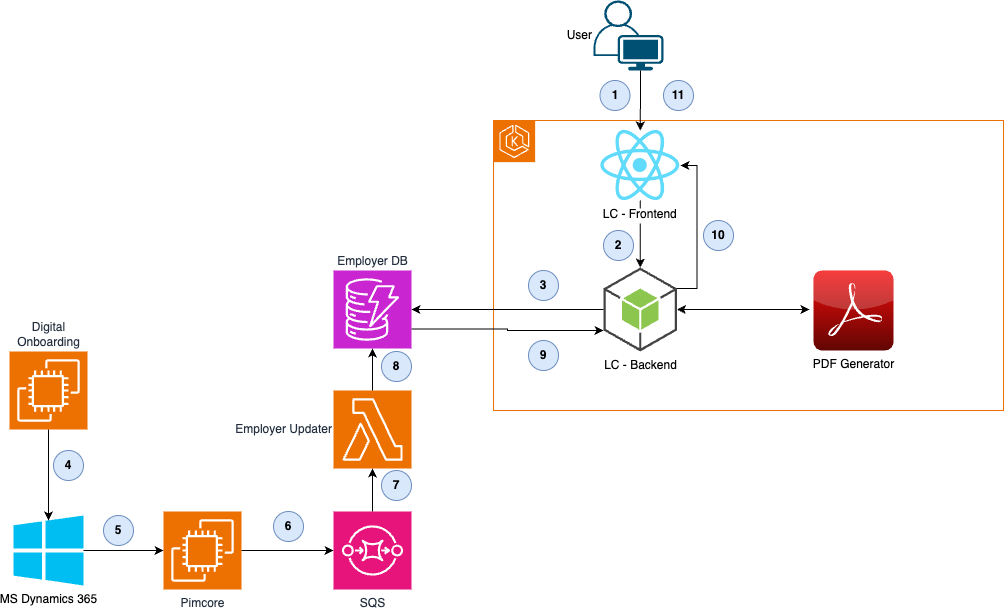
\includegraphics[scale=.3]{./assets/lc.png}
  \end{center}
\end{frame}

\begin{frame}[fragile]{Updating a microservice: the sad Atlassian case}

  \begin{columns}
    \begin{column}{0.5\textwidth}
      \begin{lstlisting}[language=json]
{
  "users": "Mike",
  "address": "Something"
}
      \end{lstlisting}
    \end{column}
    \begin{column}{0.5\textwidth}
        \begin{lstlisting}[language=json]
{
  "user": "Mike",
  "address": "Something"
}
        \end{lstlisting}
    \end{column}
  \end{columns}
\begin{center}
  
\includegraphics[scale=.4]{./assets/atlassian}
\end{center}
\end{frame}

\subsection{Test Typology}

\begin{frame}{Test Typology}
  \begin{center}
    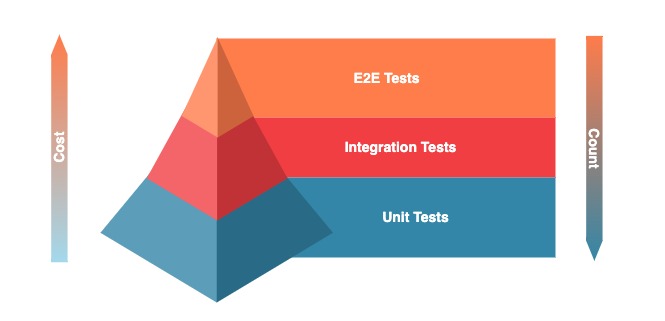
\includegraphics[scale=.6]{./assets/test_pyramid}
  \end{center}
\end{frame}

\begin{frame}{The problem with Unit Tests alone}
  \begin{itemize}
    \item Local changes, even if tested, do not assure that the system as whole is working
    \item Mocks are not guaranteed to really represent the other part of the system
  \end{itemize}
\end{frame}

\begin{frame}{The bad side of mocks}
  \begin{center}
    \animategraphics[loop,controls,scale=.5]{15}{./assets/mock/mock_problem-}{0}{232}
  \end{center}
\end{frame}

\begin{frame}{Embedded Animation}
  \begin{center}
    \animategraphics[loop,controls,scale=.28]{2}{./assets/error-propagation/errProp-}{0}{4}
  \end{center}
\end{frame}

\begin{frame}{Problem with E2E Tests}
  They're very important (\textit{qua} realistic), \textbf{but...}
  \begin{itemize}
    \item they tend to be not reproduceable locally
    \item they're hard or impossible to test some scenarios (e.g. system not available)
    \item they're expensive (time and money)
    \begin{itemize}
      \item The longer we need to find out what's wrong, the more expensive it is
    \end{itemize}
    \item Not few companies report \textit{excessive test setup}
    \item they're prone to flakiness
  \end{itemize}
\end{frame}

\begin{frame}{Architecture example}
  \begin{center}
    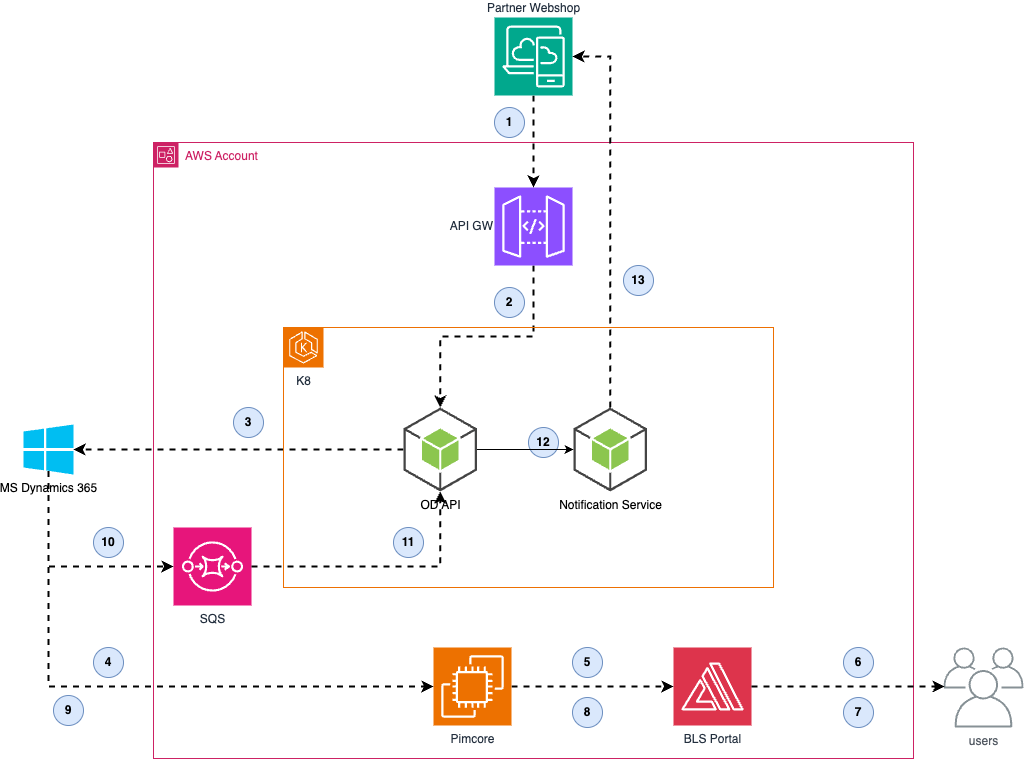
\includegraphics[scale=.3]{./assets/od.png}
  \end{center}
\end{frame}


\begin{frame}{Distributed $\ne$ Decoupled}
  \begin{center}
    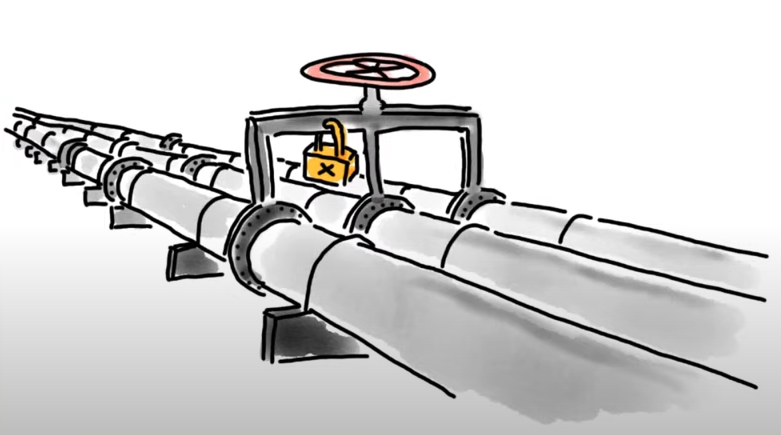
\includegraphics[scale=.43]{./assets/coupling.png}

    \textit{Is this one or three pipelines?}
  \end{center}
\end{frame}

\begin{frame}{What do we need?}
  \only<1>{

    We need a way to \textbf{test and ensure correct data exchange} between services,
    with the following characteristics:

  \vspace{.5cm}

    \begin{itemize}
      \item \textbf{Fast feedback} on changes
      \item \textbf{Confidence} in our changes
      \item \textbf{Reproducibility} of tests
      \item \textbf{Realistic} tests
      \item \textbf{Cheap} tests
      \item \textbf{Easy} to write and maintain
    \end{itemize}
  }

    \only<2>{
      \textit{Seen so far:}

      \begin{itemize}
        \item \textbf{Option A}: Mocks
        \item \textbf{Option B}: E2E / System Tests with real infrastructure
      \end{itemize}

      \textit{Is there an option C?}
    }

\end{frame}
